\section{Quantifying uncertainty on Excursion Sets implicitly defined by Gaussian processes}
\label{sec:ESEP}

In section \ref{sec:bg_and_notation} we introduce the notation used in the rest of the paper, review (co-)kriging of multivariate gaussian random fields (GRFs) and present update formulae for cokriging.
Uncertainty quantification (UQ) techniques on excursion sets of GRFs are presented in \ref{sec:set_uq}, in particular the Integrated Bernoulli Variance (IBV) and the excursion measure variance (EMV) are defined \textcolor{red}{and explicit expressions enabling their computation are derived.}
Section \ref{sec:eibv} turns to the effect of new observations on EMV and IBV. Specifically, the expected effect of the 
inclusion of a new set of observations on the EMV and IBV are considered and closed-form expressions for the expected 
uncertainty reduction are derived. Those expression form the backbone of the uncertainty reduction strategies presented in
Section \ref{sec:heuristics}.
Finally, Section \ref{Sec:UnivarEx} illustrates the application of the above concepts on a bivariate example relevant for 
sampling in the temperature and salinity application.

\medskip

Our objective is to leverage statistical tools onboard an autonomous
robotic platform to characterize a river plume, focusing on spatial
separation of cold freshwater from a river and warmer saline waters
of a fjord.

The temperature and salinity field over the domain of interest will be modeled as a bivariate gaussian random field. The \textcolor{red}{complement of the} river plume may then be characterized as an \textit{excursion set} of the field, that is, as the region of the domain for which temperature and salinity lie above some specified threshold. Our goal is then to guide the data collection process so as to improve the characterization of this set.
The methods we develop are fairly general, and not limited to the special case of two-dimensional random fields. Hence, the rest of this section will consider generic excursion sets of gaussian random fields with an arbitrary number of output dimensions.

\begin{figure}[h!] \centering
  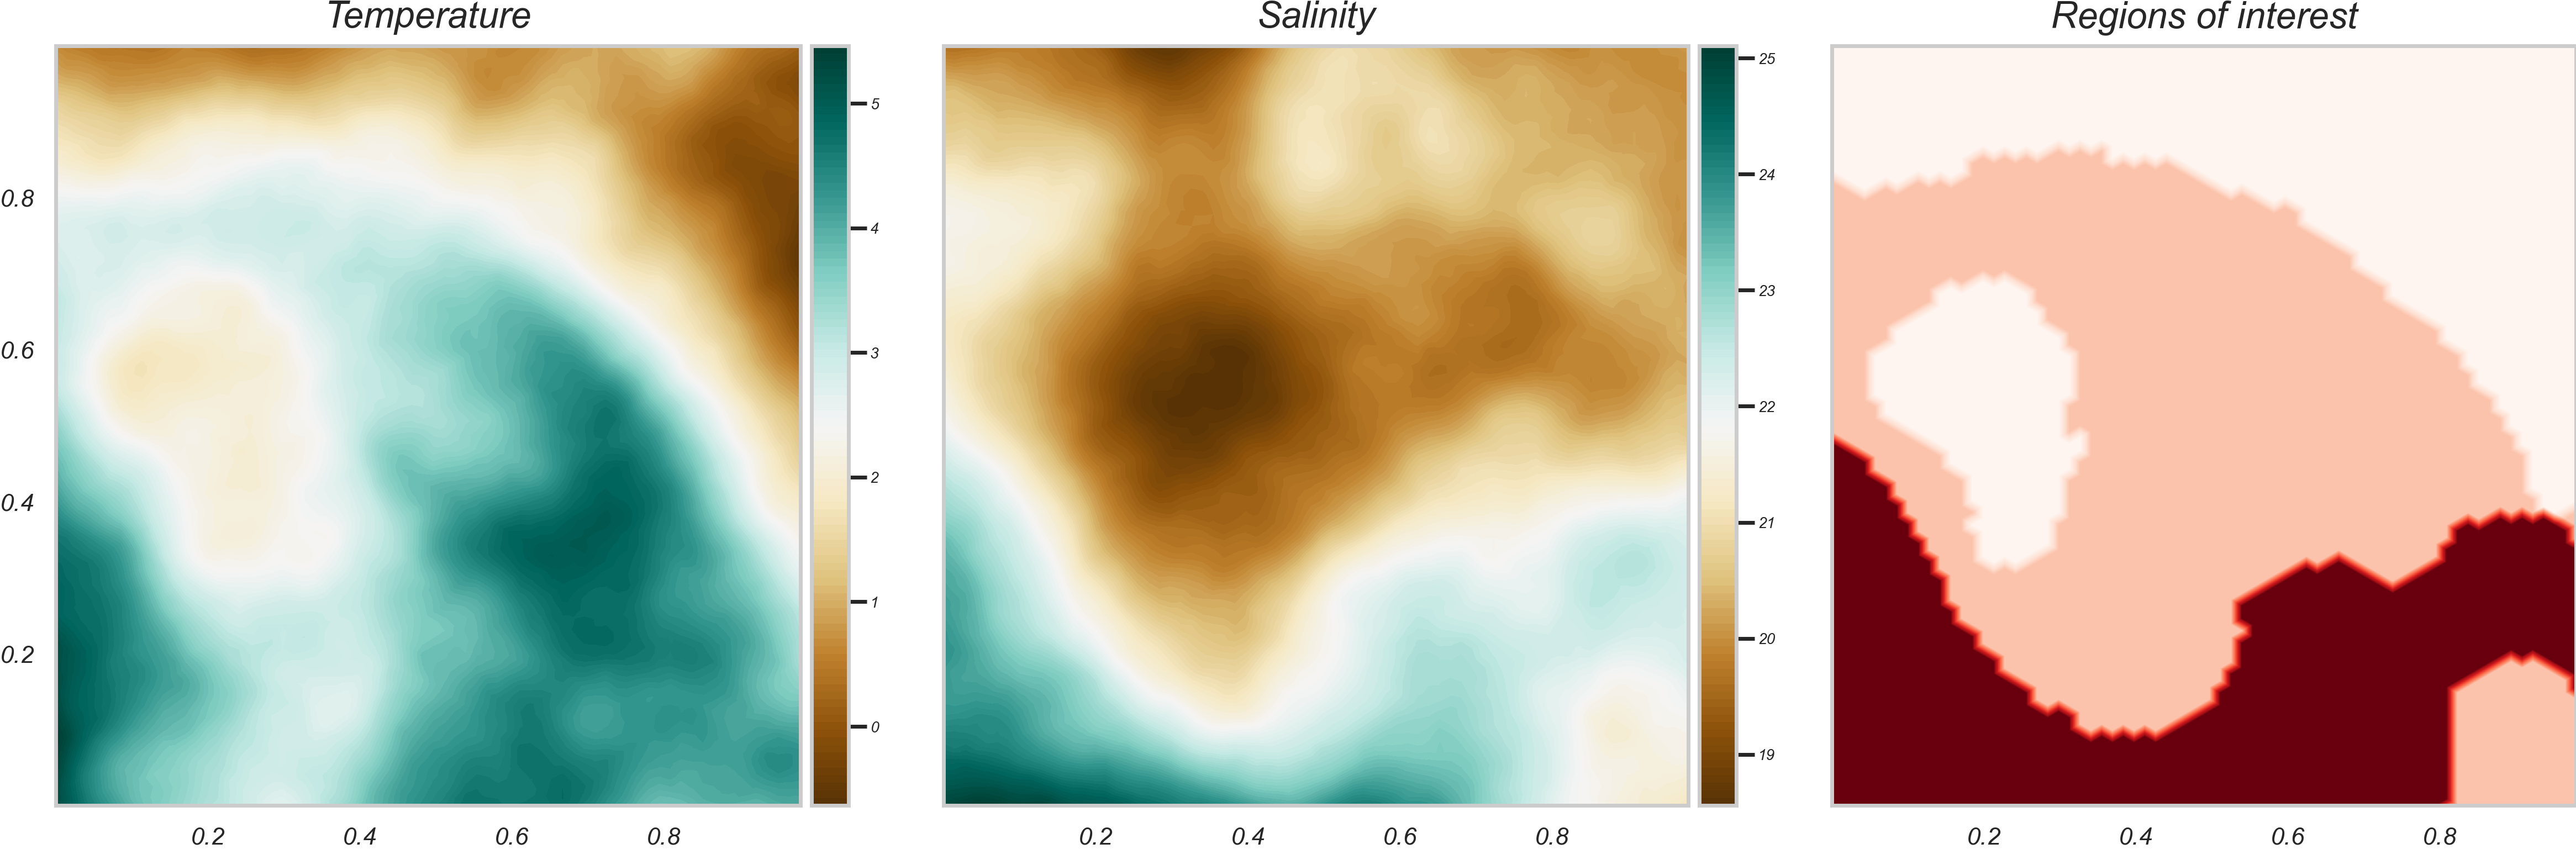
\includegraphics[width=0.99\textwidth]{Figures/example_excu_1.png}
  \caption{Realization of a bivariate GRF and excursion set above some threshold. Joint excursion in red, excursion of a single variable in white.}
\label{example_excu}
\end{figure}


Say we have an underlying phenomenon that is modeled as a $\no$-variate gaussian random field $\gp$ on some domain $\domain$, 
and we are interested in recovering the set of locations $\es$ in the domain for which the response variables (the components of $\gp$) lie in some set of specified values $\T\subset \mathbb{R}^{\no}$:
$$
\es:=\gp^{-1}(\T)=\{\x \in \mathcal{M}: \gp[\x] \in \T\}.
$$
Our goal here is to develop approaches to quantify and improve the
characterization of uncertainties on $\es$. \textcolor{red}{Alread mention how observations are included.}

If we assume that $\gp$ has
continuous trajectories (almost surely) and $T$ is closed, then
$\es$ becomes a Random Closed Set
\citep{Molchanov2005} and concepts from the theory of random sets will prove useful in characterizing the distribution of the volume of $\es$ under some measure defined on the domain.

\textcolor{red}{Is this really needed?} Note that while some aspects of the developed approaches do not call for a
specific form of $\T$, we will often stick for simplicity to the case
of orthants
($\T=(-\infty, t_1] \times \dots \times (-\infty, t_{\no}]$ where
$t_1,\dots, t_{\no} \in \R$) as this will allow efficient calculation
of several key quantities. Note that changing some $\leq$ inequalities
to $\geq$ ones would lead to immediate adaptations.


\subsection{Background, Notation and Co-Kriging}
\label{sec:bg_and_notation}
Given a random field $\gp$ and (noisy) observations of some of its components at some points in the domain, one can predict the value of the field at some unobserved location $\spatloc\in \domain$ by using the conditional mean of $\gp[\spatloc]$, conditional on the data. This process is called (co-)kriging, and kriging equations precisely tell us how to compute conditional means and covariances conditional on an arbitrary dataset.
We will here present the most general form of cokriging, where one can include several observations (batch) at a time and 
observations at a given location $s \in \domain$ may only include a subset of the components of $\gp[\spatloc]\in\mathbb{R}^{\no}$ 
(heterotopic).

\subsubsection{Notation}
In order to work at this level of generality, some notational tricks are needed. Indeed, when considering a new observation, one shall in general specify which component of the field was observed and where it was observed. This leads us to introduce the concept of \textit{generalized location}.

Letting $\gp[\spatloc,\ell]$ denote the $\ell\text{-th}$ component of $\gp[\spatloc]$, $\spatloc\in \domain$ and $\ell \in \{1\dots,p\}$, we will call \textit{generalized location} the couple $x=(\spatloc,\ell)$. Given such a generalized location notation $x$,  the notation $\gp[x]$ will be used to denote $\gp[\spatloc,\ell]$.

This slight change of notation will allow us to think of $\gp$ as a scalar-valued Gaussian random field 
indexed by $D\times \{1\dots,p\}$, which will give the co-kriging equations a particularly simple form that parallels the one of univariate kriging. Due to the naturality of the concept of \textit{generalized location}, 
we will generally use the word \textit{location}, while \textit{spatial location} will be used to stress that we are talking about a point $\spatloc \in \domain$. In the following, the letter $x$ will be reserved for generalized locations, while the letters $\spatloc$ and $\ell$ will be used for spatial locations and response indices respectively.

It turns out that the inclusion of several observations at a time (a batch) may be handled by the same equations as the 
one for a single observation, provided some notation adjustments are made. This motivates the following.



Given a dataset consisting of  $q$ observations at spatial locations $\spatloc_i \in \domain$ and response indices $l_i \in \lbrace 1, ..., \no\rbrace$, $i=1, ..., q$, we can concatenate the information needed to specify the dataset by using the notation
\begin{align*}
\bm{x}:=(\bm{\spatloc}, \bm{\ell}):= (x_1,\dots, x_q),~\text{with }x_i=(\spatloc_i,\ell_i).
\end{align*}
In general, boldface letters will be used to denote concatenated quantities corresponding to batches of observations. 
We can then also compactly denote the values of the field at those different locations by
\begin{align*}
\gp[\bm{x}]:=
\left(\gp[\spatloc_1,\ell_1], ...,
\gp[\spatloc_q,\ell_{q}]\right) \in \mathbb{R}^{q}.
\end{align*}
%
\subsubsection{Co-Kriging}
\label{sec:cokriging}
Assuming now that $n$ batches of observations are available, with respective sizes $q_1,\dots, q_n$, and that one wishes 
to predict $\gp[\bm{x}]$ for some batch of $q\geq 1$ generalized locations $\bm{x}=(\bm{\spatloc}, \bm{\ell})$, the (simple) 
cokriging mean would then amount to simple kriging with respect to a scalar-valued Gaussian random field indexed by 
$D\times \{1\dots,p\}$ and with covariance kernel $k(\bm{x}, \bm{x}')=K(\bm{\spatloc}, \bm{\spatloc}')_{\ell, \ell'}$, that is:
%
\begin{equation}
\mu_{[n]}(\bm{x})=\mu(\bm{x})+\lambda_{[n]}(\bm{x})^T (\mathbf{z}_{[n]}-\mu(\bm{x})),
\end{equation}
where $\mu$ is $Z$'s initial mean function, $\mathbf{z}_{[n]}$ stands for the ($\sum_{i=1}^n q_i$)-dimensional vector of 
observed responses of $Z$ at all considered generalized locations, and $\lambda_{[n]}(\bm{x})$ is a vector of weights 
equal to $k(\bm{x}_{[n]}, \bm{x}_{[n]})^{-1} k(\bm{x}_{[n]}, \bm{x})$ with $\bm{x}_{[n]}=(\bm{x}_1,\dots, \bm{x}_n)$, 
$k(\bm{x}_{[n]}, \bm{x}_{[n]})$ being assumed non-singular throughout the presentation. The co-kriging %(conditional) 
residual (cross-)covariance function (with respect to batches of generalized locations) can also be expressed in the same vein via
%
\begin{equation}
k_{[n]}(\bm{x},\bm{x}')=k(\bm{x},\bm{x}')-\lambda_{[n]}(\bm{x})^T k(\bm{x}_{[n]}, \bm{x}_{[n]}) \lambda_{{[n]}}(\bm{x}').
\end{equation}

\subsubsection{Co-kriging update formulae}

Let us now consider the case where co-kriging prediction of $Z$ was made with respect to $n$ batches $\bm{x}_i$ of generalized locations, concatenated again within
$\bm{x}_{[n]}=(\bm{x}_1,\dots, \bm{x}_n)$, and one wishes to update the prediction by incorporating a new vector of observations $\mathbf{z}_{n+1}$ measured at a batch of $q_{n+1} \geq 1$ generalized locations $\bm{x}_{n+1}$.
%It turns out that the concept of \textit{generalized location} makes the kriging formulae form-invariant across all dimensions. This allows us to directly adapt the 
Thanks to our representation of co-kriging in terms of simple kriging with respect to generalized locations, a strightforward adaptation of the batch-sequential kriging update formulae from \cite{Chevalier.etal2013a} delivers that
% 
\begin{equation}
\mu_{[n+1]}(\bm{x})=\mu_{[n]}(\bm{x})+\lambda_{[n+1,n+1]}(\bm{x})^T (\mathbf{z}_{n+1}-\mu(\bm{x}_{n+1})),
\end{equation}
where $\lambda_{[n+1,n+1]}(\bm{x})$ denotes the $q_{n+1}$-dimensional sub-vector extracted from
$\lambda_{[n+1]}(\bm{x})$ that corresponds to the kriging weigths associated with the last $q_{n+1}$ responses when 
predicting at $\bm{x}$ relying on all measurements until batch $(n+1)$.
%\text{th}$ batch.
%, i.e. those from the $(n+1)\text{th}$ batch of measurements conducted at $\bm{x}_{n+1}$.
Similarly, the updated co-kriging residual (cross-)covariance function then writes
\begin{equation}
k_{[n+1]}(\bm{x},\bm{x}')=k_{[n]}(\bm{x},\bm{x}')-\lambda_{[n+1,n+1]}(\bm{x})^T k_{[n]}(\bm{x}_{[n]}, \bm{x}_{[n]}) \lambda_{{[n+1,n+1]}}(\bm{x}').
\end{equation}
%\medskip
%
Let us remark that, as noted in \cite{Chevalier2015} in the case of scalar-valued fields, these update formulae naturally 
extend to Universal Kriging in second-order settings and apply without Gaussian assumption. We will now see how the latter formulae are instrumental in deriving semi-analytical formulae for stepwise uncertainty reduction criteria for 
vector-valued random fields.






\subsection{Uncertainty Quantification on Excursion Sets of multivariate Gaussian Random Fields}
\label{sec:set_uq}
We now introduce quantities that allow to quantify the uncertainty on the volume of the excursion set $\es$. Let $\mes$ be a 
(locally finite, Borel) measure  on $\domain$. We want to investigate the probability distribution 
of $\mes(\es)$ through its moments.

\medskip

Centred moments may be computed using Proposition~\ref{propo1} developed in the appendix. 
In particular, it allows to write the excursion measure variance $\emv = \operatorname{Var}[\mes(\es)]$ as an integral of the excursion probability
\begin{equation*}
\begin{split}
\emv
&=\int_{\domain^2} \mathbb{P}\left(
\gp[u]\in T, \gp[v]\in T \right)
d\mes^{\otimes}(u, v)\\
&-\left( \int_{\domain} \mathbb{P}\left(\gp[u]\in T\right) d\mes(u) \right)^2,
\end{split}
\end{equation*}
which boils down in the excursion/sojourn case where $\T=(-\infty, t_1] \times
\dots \times (-\infty, t_{\no}]$ to
\begin{equation*}
\begin{split}
\emv
%\operatorname{Var}[\mes(\es)]
&=\int_{\domain^2}
\varPhi_{2\no}
\left(
(\bt, \bt); \mu((u,v)),
K((u,v),(u,v))
\right)
\
\mathrm{d}\mes^{\otimes} %\mes
%\productMeasure
(u,v)\\
&-\left( \int_{\domain} \varPhi_{\no}\left(\bt;\mu(u), K(u)\right) d\mes(u) \right)^2,
\end{split}
\end{equation*}
%
Note that like in the case of scalar-valued fields, this quantity requires to work out an integral over $\domain^2$. In 
contrast, and still like in the scalar-valued case, the Integrated Bernoulli Variance (IBV) of \cite{Bect.etal} involves 
solely an integral on $\domain$ and can be expanded in our present settings as follows
\begin{equation*}
\begin{split}
\operatorname{IBV} %(\es) %;\mes)
&=\int_{\domain}
\mathbb{P}\left(\gp[\uu]\in T\right)(1-\mathbb{P}\left(\gp[\uu]\in T\right))
d\mes(u) \\
&=\int_{\domain}
\varPhi_{\no}\left(\bt;\mu(\uu), K(\uu)\right)
-\left(\varPhi_{\no}\left(\bt;\mu(\uu), K(\uu)\right) \right)^2
\mathrm{d}\mes(u).
\end{split}
\end{equation*}
%
Next we investigate uncertainty reduction criteria related to those indicators.






\subsection{Expected Integrated Bernoulli Variance and Excursion Measure}
\label{sec:eibv}
This section is devoted to computing the expected effect of the inclusion of new observations on the $\emv$ and $\ibv$ of the excursion set $\es$. Let us consider the same setting as in Section \ref{sec:cokriging} where $n$ batches of measurements have already been performed, and let 
$\currentExp{.}$ and $\currentProba{.}$ denote conditional expectation
and probability conditional on the first $n$ batches of observations, respectively. We want to co pute the effect of the inclusion of a new set of observations at $\bm{x}_{n+1}$ on the $\emv$ and $\ibv$.

For uncertainty functional such as $\ibv$ and $\emv$, we use a similar indexing system
with respect to a sequence of batch, and further indicate when applicable the new batch
of generalized location between parentheses; e.g., $\emv_{[n+1]}(\bm{x})$ denotes the value
of $\emv$ (a random variable, seen from ``step'' $n$, i.e. when knowing $Z$ solely at
the $n$ first generalized location batches) when adding observations at $\bm{x}$ to those
already available at step $n$.

\textcolor{red}{C.T.: This doesn't work, we cannot be that short on the definition of EIBV, it is highly unclear. I suggest we go for the following notation:
$$\operatorname{IBV}(\bm{x}; \bm{y})
$$ denotes the IBV under the current law of the field, conditioned on observing $\bm{y}$ at $\bm{x}$ (generalized, possibly batch observation). Then
$$
\operatorname{EIBV}(\bm{x}):=\mathbb{E}_{\bm{Y}}\left[\textrb{IBV}(\bm{x}; \bm{Y})\right]
$$
where $\bm{Y}$ is distributed according to the current law of $Z_{\bm{x}}$.}

\textcolor{red}{
The philosophy is the following: EIBV and EEMV are functionals of a probability distribution. Then, if not mentioned explicitly, the probability distribution will be taken to be the current law of the field. (This notation is highly efficient).}



\textcolor{red}{When one want to consider several steps, one can use $\textrm{IBV}_{n}(\bm{x}; \bm{y})$ to denote the fact that the starting point (starting probability distribution) is the law of the field at the $n$-th step $\mathbb{P}_n$ to which conditioning on $\bm{y}$ at $\bm{x}$ is added.}

\textcolor{red}{For a rigorous definition
$$
\operatorname{IBV}(\bm{x}; \bm{y}):=\int_{\domain}
\mathbb{P}\left(\gp[\uu]\in T\mid Z_{\bm{x}}=\bm{y}\right)(1-\mathbb{P}\left(\gp[\uu]\in T \mid Z_{\bm{x}}=\bm{y}\right))
d\mes(u) \\
$$
where $\mathbb{P}$ denotes the current law of the field.}



\begin{propo}
\label{propo_eibv}
Let $\eibv_{[n]}(\bm{x})=\currentExp{\ibv_{[n+1]}(\bm{x})}$ (where $\bm{x}$ plays
the role of $\bm{x}_{n+1}$) be the expected effect of adding an observation a $\bm{x}$ on the IBV.
Then we have
\begin{equation}
\begin{split}
\eibv_{[n]}(\bm{x})
&=\int_{D} \varPhi_{\no}\left(\bt;~\currentMean{\uu}, \currentCov{u, u}\right) d\mes(u)\\
&-\int_{D} \varPhi_{2\no}
\left(
\left(
\begin{matrix}
\bt-\currentMean{u}\\
\bt-\currentMean{u}
\end{matrix}
\right);
\mathbf{\Sigma}_{[n]}(\uu)
\right)
d\mes(u),
\end{split}
\end{equation}
where the matrix $\mathbf{\Sigma}_{[n]}(\uu)$ is defined as
\begin{equation*}
\begin{split}
\mathbf{\Sigma}_{[n]}(\uu)&=
\left(
\begin{matrix}
\currentCov{u, u} & \currentCov{u, u}-\futureCov{u, u}\\
\currentCov{u, u}-\futureCov{u, u} & \currentCov{u, u}
\end{matrix}
%\begin{matrix}
%\currentCov{u, u} & \Delta_{[n]}(\uu)\\
%\Delta_{[n]}(\uu) & \currentCov{u, u}
%\end{matrix}
\right).\\
\end{split}
\end{equation*}
\end{propo}

As for the expected excursion measure variance, a similar result may be derived.
\begin{propo}
\label{propo_emv}

\begin{equation*}
\begin{split}
\eemv_{[n]}(\bm{x})
&=\int_{D^2} 
\varPhi_{2\no}
\left(
(\bt, \bt); \mu((u,v)), 
K((u,v),(u,v))
\right) 
\
\mathrm{d}\mes^{\otimes} %\mes 
%\productMeasure 
(u,v)\\
&-\currentExp{
    \varPhi_{\no}\left(a_1+B_1 V; C_1\right)
    \varPhi_{\no}\left(a_2+B_2 V; C_2\right)
},
\end{split}
\end{equation*}

with $V=\gp[\bm{x}_{n+1}]-\currentMean{\bm{x}_{n+1}} \sim \mathcal{N}(0_{q_{n+1}},k_{[n]}(\bm{x}_{n+1},\bm{x}_{n+1}))$ and $a_1=\bt-\currentMean{\uu}$,
$B_1=-\lambda_{[n+1,n+1]}(\uu)^T$, $a_2=\bt-\currentMean{\vv}$, $B_2=-\lambda_{[n+1,n+1]}(\vv)^T$.

This integrand finally boils down to an evaluation of the $2\no$-dimensional Gaussian CDF by
Proposition~\ref{propo3}. Details are omitted here for brevity as we did not implement further
this criterion that requires numerical integration over $\domain^2$.
\end{propo}


Note that the calculation of the multivariate Gaussian cumulative distribution
may be done effectively using code such as that of
\cite{genz2009computation}. 

\textcolor{red}{Do we really want to keep this?}
A critical element in the derivation of a closed-form for the EIBV is
that the conditional mean in the cokriging equations is a linear
(affine) function of the data $\by_d$ and the covariance is not a
function of the data. This in turn means that the probabilities in Eq.
\eqref{eq:post_ep} involve inequality statements for linear
combinations of Gaussian variables. Related closed-form solutions have
been noted in similar contexts \citep{bhattacharjya2013value,
  chevalier2014fast,stroh}, but not generalized to our situation with
random sets for vector-valued GPs.











\subsection{Expected Bernoulli Variance on a two dimensional Example}
\label{Sec:UnivarEx}
We illustrate the EBV associated to different designs on a simple bivariate example. The example mimics our river plume application and hence the first and second component of the random field will be called \textit{temperature} and \textit{salinity} for illustrative purpose. Effects of the hyperparameters of the GRF prior on the excursion probabilities will also be studied. For simplicity, we begin with a \textit{pointwise} example, considering a single bivariate gaussian distribution (no spatiality).

\subsubsection{A pointwise study}
Say we want to study the excursion probability of a bivariate gaussian, where the excursion set is defined as
\[
\Gamma := \lbrace \spatloc \in \domain: Z_{\spatloc, 1} \geq t_1, Z_{\spatloc, 2}\geq t_2\rbrace
\]
and the thresholds are set equal to the mean; $\mu_1=t_1=5^o C$ for temperature and  $\mu_2=t_2=30$ mg/l for salinity, and we play with the temperature and salinity correlation and variances to study the effect on the EP and expected Bernoulli variance.

Fig. \ref{illus_bivarDens} shows contour plots of three different
densities with increasing correlation $\gamma$ between temperature and
salinity. 
\begin{figure}[h!] \centering
  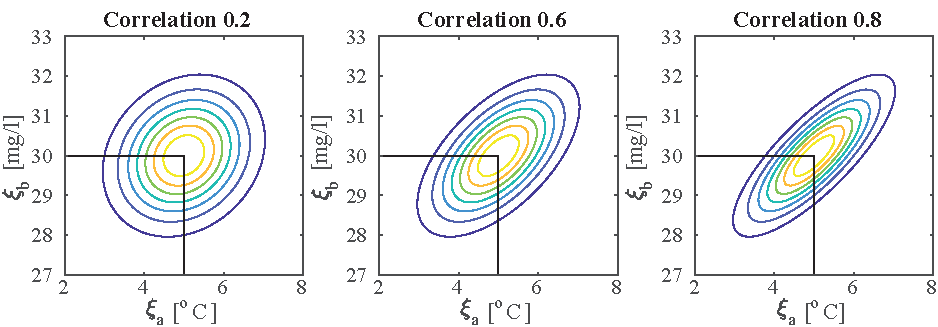
\includegraphics[width=0.99\textwidth]{Figures/illus_bivar.pdf}
  \caption{Density contour plots with different correlations between
    temperature and salinity. The densities have unit variance and the
    thresholds are identical to the mean values $5^o C$ and
    $30 mg/l$. X-axis is temperature and y-axis is salinity.}
\label{illus_bivarDens}
\end{figure}
The displayed densities have unit standard deviations for both
temperature and salinity, but we also study the effect of doubling the
standard deviations.

Table \ref{tab:sim_rhoab} shows the initial EPs and the associated
Bernoulli variance (second row) for the examples indicated in Fig.
\ref{illus_bivarDens}. The EPs increase with the correlation as there
is a strong tendency to have concurrently low temperature and salinity. The Bernoulli variance is similarly large for high
correlations. EPs and Bernoulli variances are the same for standard
deviation $1$ or $2$, which implies that high variability in
temperature and salinity is not captured in the $p(1-p)$ expression.

\begin{table}[!h] \centering \caption{EP and Bernoulli variance for
    different correlations and variances (top rows), and expected
    Bernoulli variances for both temperature and salinity data $\by$ and 
    temperature $y_2$ (bottom rows).}
  \begin{tabular}{c|ccc|ccc}
 &\multicolumn{3}{c}{$\sigma_1=\sigma_2=1$} & \multicolumn{3}{c}{$\sigma_1=\sigma_2=2$} \\
\hline
Correlation $\gamma$ & 0.2 & 0.6 & 0.8 & 0.2 & 0.6 & 0.8 \\
\hline
$p$ & 0.28 & 0.35 & 0.40 & 0.28 & 0.35 & 0.40 \\ 
$p(1-p)$ & 0.20 & 0.23 & 0.24 & 0.20 & 0.23 & 0.24 \\ 
EIBV, Temp and Salinity data & 0.092 & 0.089 & 0.085 & 0.052 & 0.051 & 0.049 \\ 
EIBV, Temperature data only & 0.151 & 0.138 & 0.123 & 0.137 & 0.114 & 0.093 \\ 
\hline
\end{tabular}
\label{tab:sim_rhoab}
\end{table}

Table \ref{tab:sim_rhoab} (bottom two rows) shows results of expected
Bernoulli variance calculations. This is presented for a design
gathering both data types, and for a design with temperature
measurements alone. When both data are gathered, the measurement model is
$(Y_{d,1},Y_{d,2})^t=(Z_1,Z_2)^t+\bepsilon$, with $\bepsilon \sim N(0,0.5^2I_2)$, while $Y_d=Z_1+\epsilon$, $\epsilon \sim N(0,0.5^2)$ when only temperature is measured.
For this illustration, Table \ref{tab:sim_rhoab} shows that the
expected Bernoulli variance gets lower with larger standard deviations
$\sigma_1$ and $\sigma_2$ (right columns). The reduction of Bernoulli
variance is largest for the cases with high correlation
$\gamma$. Albeit smaller, there is also uncertainty reduction when
only temperature is measured (bottom row), especially when temperature
and salinity are highly correlated. When correlation is low
($\gamma=0.2$), there is little information about salinity in the
temperature data, and therefore less uncertainty reduction. In an
application with fresh cold water from a river source, the temperature
and salinity variables will not only be interdependent, but will also
likely show dependence in the spatial dimension. This in turn will
impact the design criteria when we evaluate the information measure by
integrating over several locations (Section \ref{sec:simulations}).

\subsubsection{Including Spatiality}
INTRODUCTORY SENTENCE.
The class of GRF model we will consider in the article will generally have a linear trend
\begin{align*}
\mu(s)=\mathbb{E}\left[\begin{pmatrix}
Z_{s, 1}\\ Z_{s, 2}
\end{pmatrix}\right] &= \beta_0 + \beta_1 s
\end{align*}
with $\beta_0$ a two dimensional vector and $\beta_1$ a $2\times 2$ matrix. We will only consider covariance models of separable type
\begin{align*}
\textrm{Cov}\left(Z_{s, i}, Z_{u, j}\right) &= k(s, u) \gamma(i, j),~ \gamma(i, j) = \begin{cases} \sigma_l^2,~ i=j\\
   \gamma_0 \sigma_i \sigma_j,~i\neq j
        \end{cases}
\end{align*}
where $k(., .)$ is one of the traditional spatial covariance kernel (exponential, Mat\'{e}rn, ...) and $\gamma$ defines the cross-covariance structure.

In the accompanying Python code, these modeling assumptions can be
generalized to anisotropic covariance and changing variance levels
across the spatial domain. One can hence, easily run the code to see
if different models result in other sampling designs. Anisotropy and
non-stationary variance are both relevant for the setting with river
plumes, but in practice this requires more parameters to be
specified. With extensive data and prior knowledge, one could also
possibly fit and estimate parameters of more complex multivariate
spatial covariance functions
\citep{gneiting2010matern,genton2015cross}, but that is outside the
scope of the current paper.

In the rest of this section, we will consider a GRF with mean and covariance structure as above and parameters
\begin{align*}
\beta_0 = \begin{pmatrix}
5.8\\ 24.0
\end{pmatrix}, ~ \beta_1 = \begin{pmatrix}
0.0 & -4.0\\
0.0 & -3.8
\end{pmatrix},~ \sigma_1 = \sigma_2 = 2.25, ~ \gamma_0 = 0.2
\end{align*}
and the spatial covariance is given by a Mat\'{e}rn 3/2 kernel with unit variance and range parameter $\lambda=0.5$.
One realization of this GRF is shown in Fig. \ref{example_excu}.

We now study how the expected Bernoulli variance eq.\ref{eq:eibv} associated to data collection at a point changes if only one of the two components of the field is observed. We first draw a realization of the GRF defined above and use it as ground-truth to mimick the real data-collection process. A first data collection step is performed at the location in green, and the data is used to update the GRF model. The expected Bernoulli variance reduction (at each grid point) that would result from observing only one component, or both at the next grid point upwards is then computed an shown in Fig.\ref{fig:ebv_comp}.

\begin{figure}[h!] \centering
  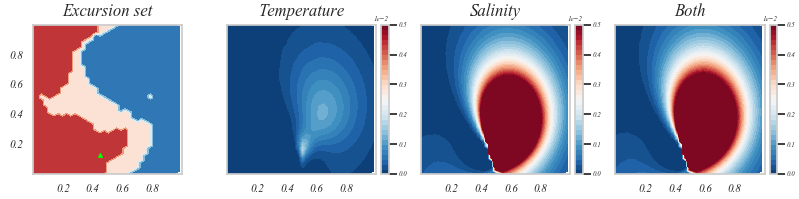
\includegraphics[width=0.99\textwidth]{Figures/ebv_comp.png}
  \caption{Pointwise Bernoulli variance reduction for observation of a single or both components of the random field at one location. Data collection locations in green. True excursion set in red. Places where only one response is above threshold are depicted in pink}
\label{fig:ebv_comp}
\end{figure}

Note that plotting the Bernoulli variance reduction at each point might also be used to compare different data collection plans. For example, Fig. \ref{fig:ebv_comp} shows the expected Bernoulli variance reduction associated to a data collection plan along a straight upwards line (static north) and the one associated to a straight horizontal line (static east). Both expectations are computed according to the a priori distribution of the GRF (i.e. no observations have been included yet).

\begin{figure}[h!] \centering
  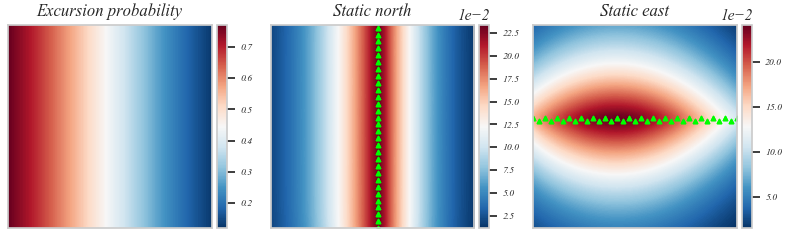
\includegraphics[width=0.99\textwidth]{Figures/ebv_north_vs_east.png}
  \caption{Pointwise Bernoulli variance reduction for two different observation plans. Data collection locations in green. True excursion set is in red. Places where only one response is above threshold are depicted in pink.}
\label{fig:ebv_north_vs_east}
\end{figure}

\begin{remark}
In all the above examples, the spatial domain $\domain$ has been discretized to a set of $n$ grid
locations $\mathcal{M}_g = \{\x_i, i=1,\ldots,n \}$, where each cell
has area $\Delta$; the same grid is used for the waypoint graph for
possible design locations. The EIBV is approximated by sums over all
grid cells.
\end{remark}